\documentclass[conference]{IEEEtran}
\usepackage{cite}
\usepackage{amsmath,amssymb,amsfonts}
\usepackage{algorithmic}
\usepackage{graphicx}
\usepackage{textcomp}
\usepackage{xcolor}
\def\BibTeX{{\rm B\kern-.05em{\sc i\kern-.025em b}\kern-.08em T\kern-.1667em\lower.7ex\hbox{E}\kern-.125emX}}
\begin{document}

    \title{Accelerating AI: A Comparative Analysis of GPUs, TPUs, and their Performance}

    \author{\IEEEauthorblockN{Abel Haris Harsono\IEEEauthorrefmark{1},
        Arnav Varshney\IEEEauthorrefmark{2}, Filbert David Tejalaksana\IEEEauthorrefmark{3}}
    \IEEEauthorblockA{\textit{Department of Electrical and Electronic Engineering} \\
    \textit{The University of Hong Kong}\\
    Hong Kong \\
    \{ u3583434\IEEEauthorrefmark{1}, arnav\IEEEauthorrefmark{2}, f1lbert\IEEEauthorrefmark{3} \}@connect.hku.hk}
    }

    \maketitle

    \begin{abstract}
        This document is a model and instructions for \LaTeX.
        This and the IEEEtran.cls file define the components of your paper [title, text, heads, etc.].
        *CRITICAL: Do Not Use Symbols, Special Characters, Footnotes,
        or Math in Paper Title or Abstract.
    \end{abstract}

    \begin{IEEEkeywords}
        component, formatting, style, styling, insert
    \end{IEEEkeywords}


    \section{Introduction}

    \{Generated from GPT; a placeholder\}
    Deep learning algorithms, particularly neural networks with millions of parameters, have demonstrated exceptional capabilities in solving complex tasks such as image recognition, speech synthesis, and language translation.
    However, the computational demands of training and deploying these models pose significant challenges for traditional CPUs (Central Processing Units) and even GPUs.
    To address this issue, specialized hardware accelerators specifically designed for deep learning workloads have gained immense popularity.

    Google's Tensor Processing Unit (TPU) and Nvidia's A100 GPU have emerged as two prominent contenders in the market, representing cutting-edge architectures tailored to accelerate deep learning tasks.
    While both platforms aim to deliver high performance, they adopt different approaches to achieve optimal efficiency.
    The TPU is a custom-built integrated circuit designed by Google, while the A100 leverages the latest GPU architecture from Nvidia.
    Understanding the unique features and trade-offs of each platform is crucial for researchers and practitioners to make informed decisions when selecting hardware accelerators for their deep learning applications.

    This paper presents a detailed comparative analysis of Google's TPU and Nvidia's A100, focusing on their architectural characteristics, computational capabilities, memory systems, and power efficiency.
    Furthermore, we explore their performance across a range of deep learning benchmarks and discuss the impact of each platform's design choices on the overall performance and usability.
    The analysis considers factors such as peak performance, memory bandwidth, precision support, and software ecosystem to provide a comprehensive evaluation of the strengths and weaknesses of each platform.

    The remainder of this document is structured as follows: Section II provides an overview of the architectural features of Google's TPU and Nvidia's A100.
    Section III discusses the performance metrics and benchmarks used to evaluate the platforms.
    Section IV presents a comparative analysis of the TPU and A100, highlighting their similarities and differences.
    Section V discusses the implications of the findings and provides recommendations for selecting the most suitable platform for different deep learning applications.
    Finally, Section VI concludes the paper and outlines potential avenues for future research in the field of deep learning hardware accelerators.

    In summary, this paper aims to contribute to the body of knowledge surrounding hardware accelerators for deep learning by providing an in-depth analysis of Google's TPU and Nvidia's A100.
    The results of this comparative study will aid researchers, developers, and practitioners in making informed decisions when selecting the most appropriate platform for their specific deep learning requirements.


    \section{Nvidia A100 Tensor Core GPU}

    \subsection{Introduction}
    Deep neural networks are usually composed of sequential interconnected layers.
    This structure allows for extreme parallelism as computations are broken into smaller chunks, albeit still dependent on its previous layers.
    Each layer in a neural network takes in an activation tensor as well as a weight tensor.
    An activation tensor represents the output of a single node in the layer, while a weight tensor represents the learning parameters in the network.
    The computation between the two tensors involves a mathematical expression similar to matrix multiplications, outputting an activation tensor fed on to the next layer.

    \subsection{SM Core}
    The structure of the A100's SM core works via a 5 step process.
    The A100's memory hierarchy starts with the off-chip DRAM\@.
    The DRAM provides global access to resources for the SMs.
    Data is first loaded from the DRAM into the on-chip L2 cache, acting as a large pool of shared memory accessible by all SMs.
    An asynchronous instruction will then be used to partition the data resource for SMEM usage individually and concurrently without blocking the main execution pipeline.
    Think of the instruction as an asynchronous implicit duplicate instruction that allows data to be loaded directly from the main memory into a shared memory.
    The SMEM connects to the tensor cores via a register file, which acts as a high-speed buffer location, allowing tensor cores to efficiently read and write data to and from the SMEM\@.

    \begin{figure}[htbp!]
        \centerline{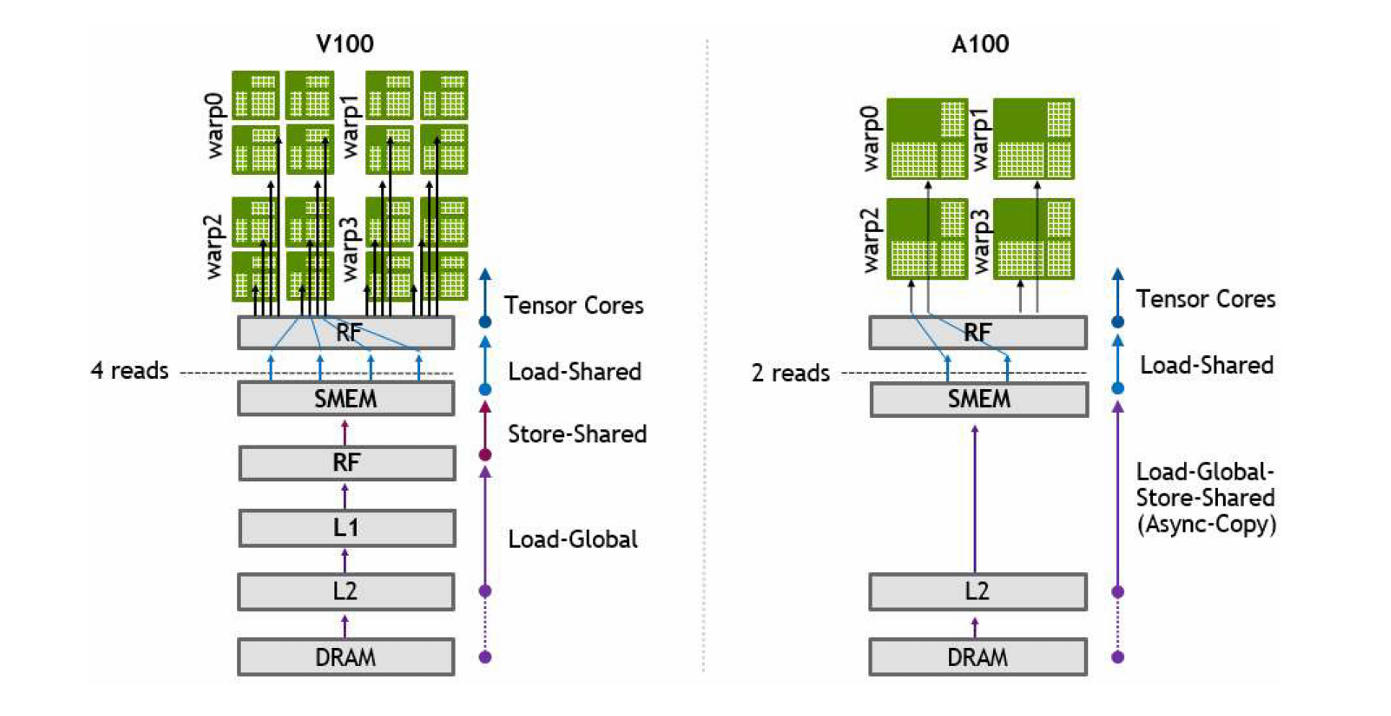
\includegraphics[width=0.5\textwidth]{images/gpu_structure}}
        \caption{V100 vs A100 structure.}
        \label{fig}
    \end{figure}

    To give context to the particular design of the A100, we can look at the V100, a GPU preceding the A100.
    The V100 works with a 7 step process.
    In the same fashion, data is loaded into an L2 cache from the DRAM, but instead of a direct connection to the SMEM, the V100 requires an additional layer of caching.
    By having a dedicated L1 cache per SM, the V100 can better utilize the available memory bandwidth.
    Each SM can access its own L1 cache independently, reducing contention and improving overall throughput.
    The V100 lacks the asynchronous load and store instruction in its instruction set, thus it requires an explicit write instruction to the SMEM to transfer data.

    \begin{figure}[htbp!]
        \centerline{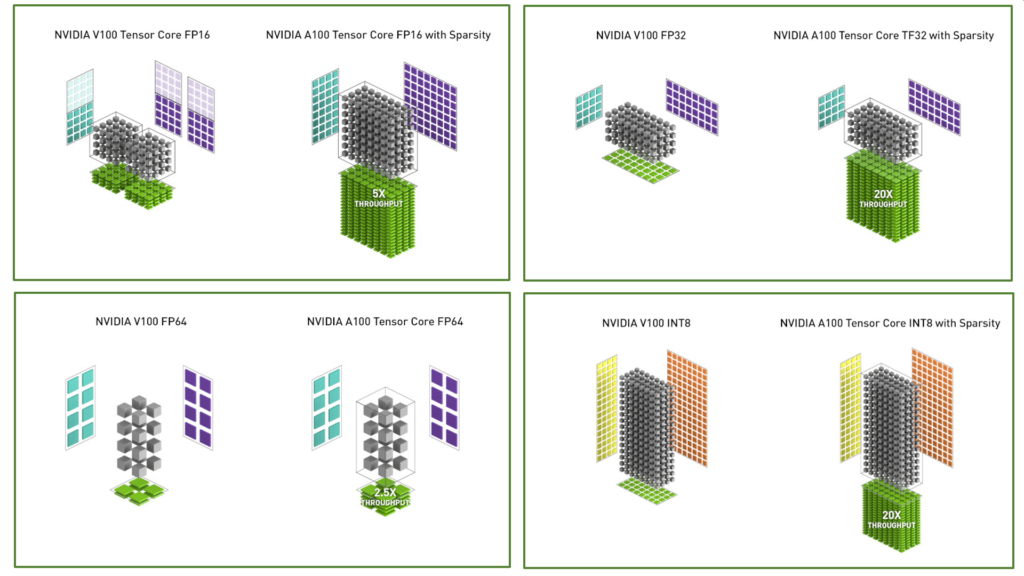
\includegraphics[width=0.5\textwidth]{images/gpu_sparsity}}
        \caption{V100 vs A100 sparsity.}
        \label{fig}
    \end{figure}

    The simplification of the V100 design into the A100 is actually caused by the massive throughput of the tensor core itself.
    In both the V100 and A100 designs, the neural network workloads break down each tile into four smaller workable tiles that can be processed in parallel.
    Each of those tiles will then be processed by a 32-thread warp.
    The V100 tensor cores were designed to work with 8-thread granularity, meaning each tensor core operation would process 8 threads simultaneously, while the A100 works with 32-thread granularity.
    The figure above compares the V100’s and A100’s standard operation with multiple data types.
    The data types given such as TF32 and TF16 are much more efficient in using tensor accelerated math than its floating point counterparts, having the same exponent range, albeit less precision.

    The 8-thread granularity of the V100's individual network tiles forces it to have a proportionally higher number of load from memory and lower bandwidth in the SMEM, since the 8-thread granularity combined with the fact that data has to move from the L2 cache, to the L1 cache and then to the SMEM, results in higher number of memory access operations per tile.
    Reorganizing the A100 to utilize 32-thread granularity allows it to process a full warp of 32 threads all at once, coupled with improvements in memory access, changed the memory access count from 1 L1 read, 1 SMEM write and 4 SMEM reads into just two SMEM reads per tile.
    This reduction in memory access simplifies the data path by relying more on the higher bandwidth SMEM connecting directly without intermediary storage.

    \subsection{L2 Cache}
    An L2 cache in the A100 is a globally shared resource for the SMs.The A100 divides its L2 cache partitions into two distinct partitions: high bandwidth access and low latency memory access.
    The cache allows for a substantial increase in machine learning workloads, with larger datasets and models now being able to be cached and repeatedly hit, contrasting to the V100 requiring slower reading and writing, from and to the HBM2 memory.
    The prime enabler of the partition is the L2 Cache Residency Control.
    The residency control basically enables a partition of the cache to be used for persistent data access.The A100 employs two key mechanisms to manage persistent accesses to the L2 cache:

    \subsubsection{Address-based Persistent Window} Specified address range or “window” will be cached instead of caching a single address and designated to be resident.
    Read and write access would be a guaranteed hit in the window.
    This method benefits from array-like or consecutive structures such as neural network parameters.

    \subsubsection{Per-Memory-Operation Persistent Control} The residency control exposes control over Individual memory accesses to be tagged as persistent by the user, otherwise individual access will not be tagged.
    These two persistent access mechanisms work together to optimize the utilization of the L2 cache.
    Cache Residency only allows cache tagging when there are ``group access`` to a particular address at a close time, while individual memory access will bypass cache, or can be controlled directly by user to persist.

    \subsection{DRAM}
    The A100 DRAM uses HBM2 memory technology.
    The DRAM consists of 5 of these HBM2 memory stacks, laid vertically and connected to the GPU die via high-speed interconnects.
    The tight integration reduces memory latency, power consumption, and its compact stack design aids in the memory having a smaller physical footprint compared to traditional GDDR memory.

    \subsection{Closing}
    The NVIDIA A100 GPU marks a significant advancement in GPU architecture, leveraging innovative hardware designs.
    From streamlining its preceding 7 step process of the SM core to a 5 step process, to including compression and residency algorithms to the cache, and introducing asynchronous partitioning instruction to enable direct data transfer to high bandwidth SMEM\@.


    \section{Tensor Processing Unit}

    \subsection{Introduction}
    A Tensor Processing Unit (TPU), similar to a Graphical Processing Unit (GPU) and Central Processing Unit (CPU), is a computing device with the difference being the focus of their activities.
    While GPUs and CPUs are considered general purpose, TPUs are special purpose; they are built to accelerate performance of ML related applications particularly in linear algebraic processes involving matrices.
    They cannot do much else, at least not efficiently.
    As of now, the TPU has iterated to its 5th version but for the purposes of this work, we will mention only TPUv4 and highlight the important features it has.

    \subsection{Structure}
    There are 2 main components of a TPU chip: High Bandwidth Memory (HBM) and the Tensor Cores (TC).
    The HBM is an on-chip memory allowing for larger models and bigger batch sizes.
    The TCs on the other hand consists of many multiply-accumulators; the special hardware that allows for an increase in speed for matrix-related operations.
    These multiply-accumulators are all arranged in an array-like structure called the systolic array structure.

    Google’s TPU machine consists of thousands of these TPU chips (as of TPUv4, there are 4096 chips placed inside).
    Within the machine itself, the chips are arranged physically as a cube but the inner networking between the chips would form a torus.
    This is actually only the default configuration.
    Users are able to define their own topology (in terms of networking).

    The TPU works by first loading parameters from the HBM, load them into individual multiply-accumulators and then load the data to one layer of the array-like architecture and let the results of one computation feed the next one, and so on.
    It’s akin to how a ripple-carry adder works.

    \subsection{TPUv4}
    These features are all common amongst the different iterations of the TPU\@.
    If so, then what is so important about the TPUv4?
    The main improvements introduced handles around the subject of scale and reliability using google's very own advancement in optical switches.
    Additionally, just as any other kind of iteration, the tpuv4 also improves certain aspects of the system i.e.
    On the dealing with storage of embeddings by introducing the appropriate hardware architectures and introducing a way that allows for a better compatibility between hardware and the model.

    \subsubsection{Reconfigurable Optical Switches}
    As mentioned, the TPUv4 has 4096 TPU chips.
    This number may seem insignificant to some, but we can compare that to the previous version’s (TPUv3) 1024 chips.
    The sheer size of the TPUv4 renders electrical switches useless due to “electrical interconnect” limitations.
    To solve this, optical switches were used.
    In particular, Google's Palomar Optically Configurable Switches (OCS).
    They are based on Micro-Electro-Mechanical Systems that can send light both ways in a fiber by employing what's called a ``circulator``.

    \begin{figure}[htbp!]
        \centerline{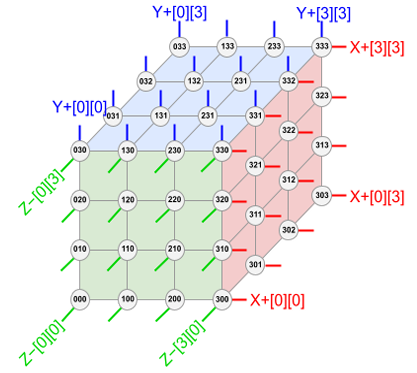
\includegraphics[width=0.2\textwidth]{images/tpu_cube}
        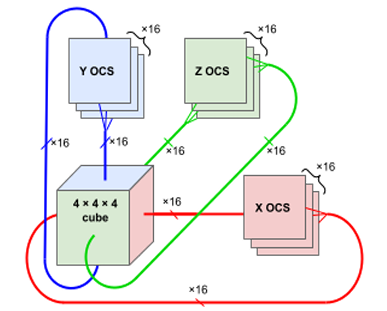
\includegraphics[width=0.2\textwidth]{images/tpu_connectivity}}
        \caption{OCS Architecture.}
        \label{fig}
    \end{figure}

    The figure illustrates how the OCSs are connected.
    This cube, a 4 x 4 x 4, is part of the TPU machine that consists of many TPU chips that must be connected to the OCS (We consider a cubic arrangement of 64 chips due to nicer bisection bandwidth and for convenience in storage).
    The way we connect them together is by connecting each side’s chips to the OCS and the opposite side of that side connected to the same OCS\@.
    In total, for TPUv4, there are typically 3 * 16 = 48 OCSs for a single machine.

    The OCS brings a multitude of benefits.
    The first is availability and deployment benefits.
    Being flexible and having better performance allows TPUv4 to still provide good services although some hosts of the system may not be available.
    And because the OCSs bring some sort of independence to the system (particularly, it made each rack of the chips more independent), not all chips are needed to ensure operability.

    Then, the most obvious one, configurable.
    The OCS greatly simplifies scheduling and networking within the system due to its great switching speed.
    For instance, it no longer has to search for many contiguous chips during scheduling and it allows modularity between users (the whole system can cater to multiple users) which enhances security.
    Finally, foreshadowed before, the whole system can be reconfigured to your own topological needs, like exploiting parallelisms, as ``rewiring`` the system mostly involve reprogramming the routes of the OCS\@.

    \subsubsection{SparseCore}
    Like any other computers dealing with ML, This one is for dealing with embedding.
    In particular, where to store the lookup tables from the embedding process.
    The main problem here is that the lookup operations will causes a bottleneck for the chips due to memory accesses, inter chip communication, etc.
    As they are more suited for dense arithmetic operation.

    In this context, there were 2 possible solutions: either put it in the host’s CPU or put it in the tensor cores themselves.
    The Host’s CPU approach would introduce a bottleneck during the next iterations by Ahmdal’s law; in comparison, there is a 4:1 TPUv4 to host CPU ratio.
    On the other hand putting it in the TC would be suboptimal due to their nature.
    A way out of this is to utilize both the HBM and the dedicated Inter-Core Interconnect (ICI) network which are embedded in the chips.
    With these in mind, comes SparseCore (SC).
    It’s an additional hardware put in the machine for dealing with embedding training.
    SC utilizes the HBM and a dedicated ICI network while operating in a sea of cores configuration creating a flat, globally addressable memory space.

    \subsubsection{Platform-Aware Neural Architecture Search}
    Platform-Aware Neural Architecture Search or PA-NAS has a goal to configure both the ML model and the TPU topology to benefit from each other as much as possible.
    In particular, with the mention of SC, a model in the TPU might need to use both SC and TC efficiently.
    PA-NAS optimizes operations related to this to achieve “pareto-optimal performance and quality”.


    \section{Contribution Statement}
    \begin{itemize}
        \item Abel Haris Harsono: 33.3\%
        \item Arnav Varshney: 33.3\%
        \item Filbert David Tejalaksana: 33.3\%
    \end{itemize}
\end{document}
